
\lhead[\chaptername~\thechapter]{\rightmark}

\rhead[\leftmark]{}

\lfoot[\thepage]{}

\cfoot{}

\rfoot[]{\thepage}

\chapter{Implementation in \emph{R}\label{chap:Implementation}}

\begin{comment}
Both R and Python are powerful programming languages for data analysis.
Python has been known as a general purpose language with an easy to
understand syntax. It emphasizes on code readability and has a gentle
learning curve. R is developed by and for statistician. It provides
a huge number of essential packages in statistics, and even starts
to expand its package to different fields. R also has a strong reputation
for data visualization. However, in terms of computation, R still
cannot compete with Python which is built specifically for the computer
programming. 

With strengths and weaknesses between R and Python described earlier,
R is chosen to be used in this study. R offers more implemented algorithms
to solve the problem at hand. Moreover, an effective visualization
helps analyst and user to understand more about their data especially
for the complex one. Visualizing data is useful in many ways such
as uncover new patterns, identify some factors, and get an overall
trend. R proves to be a good choice as it provides a great feature
in creating an interactive graphic.
\end{comment}


\section{EventsPerSec\label{sec:EventsPerSec}}

The \emph{EventsPerSec} variable contains several local events in
the test case which are separated by a tab character. A function to
split tab-separated values in the field into columns is described
by the following steps.

\begin{algorithm}[h]
\caption{Extract local events in EventsPerSec}

\begin{algorithmic}[1] 
\For{each test case}
\State{Split the vector of local events with its value into elements} 
\For{each element} 
\State{Split the element into the local event and the value}
\If{the column of the local event exists in the data}
\State{Insert value}
\Else{}
\State{Create new column for this local event and insert its value}
\EndIf
\EndFor
\EndFor
\State{Replace missing value with zero}
\end{algorithmic}
\end{algorithm}


\section{MSwM Package\label{sec:MSwM-Package}}

A \emph{MSwM} package in R \citep{mswm} is mainly used to perform
an univariate autoregressive Markov switching model for linear and
generalized models. The package implements an Expectation-Maximization
(E-M) algorithm to fit the Markov switching model. 

Code was further implemented, and some modifications were also made
in the function to handle warnings and errors produced when fitting
the model. These modifications are described in more details here.

\paragraph*{Non-switching effect}

When setting variance to have a non-switching effect, a function generates
a warning. This issue is caused by a minor mistake in the code. 

\paragraph{Non-invertible Hessian}

The package uses a Hessian, a matrix of second order partial derivatives
with respect to parameters, for a numerical optimization. In some
cases, the Hessian matrix will not be invertible as the matrix is
singular. Consequently, the function cannot compute the standard error
of estimated parameters. It is assumed that the singularity is coming
from numerics issue i.e., the matrix is not singular but computationally
it is. This non-invertible Hessian is solved by using generalized
inverse (or pseudoinverse) procedure \citep{gill2004your}. 

\paragraph*{Plots}

Two more plots for visualizing the results have been added to the
package. Name of functions and descriptions are provided below. 
\begin{itemize}
\item \code{plotSmo(object)} 

Plot of smoothed probabilities with different states

Description: Creates a plot that shows the smoothed probabilities
for all the states.
\item \code{plotArea(object)} 

Plot of response variable with state specifications

Description: Create a plot that shows the periods where the variable
is in the specific states.
\end{itemize}

\paragraph*{Categorical variable}

The package does not appear to work well with categorical predictor
variables. Hence, a further implementation in the code for handling
with categorical variables is done. R refers to categorical variables
as factors. Most of the time, an order of the factor does not matter
in the study. However, sometimes the order of the factor is of interest
in the analysis and needs to be specified for the purpose of comparison
or obtaining a meaningful interpretation. 

\begin{comment}
finding the highest occurrence and set it to be reference level
\end{comment}


\paragraph*{NA coefficients}

When performing the Markov switching model, a function in the package
first randomly divides the data into different subsets, and then separately
fit the model to each subset to get initial coefficients in each state.
These coefficients are later used for further analysis e.g., computing
condition means, conditional residuals of the model, and likelihood
of the parameters for each state.

It is worth noting that the function computes conditional means for
each state by using matrix multiplication $\ensuremath{\hat{y}=X\hat{\beta}}$.
Therefore, if NAs exist in the coefficient matrix $\hat{\beta}$,
these conditional means $\hat{y}$ will become NAs, and so does conditional
residuals and likelihood of the parameters.

The main reason that generated this NA coefficient issue is due to
the randomness in partitioning the data. The issue frequently occurs
with a categorical variable because each categorical variable has
its own number of levels. The following situations listed below are
what generated an error and NA coefficient:
\begin{itemize}
\item A variable in a subset contains the same value in all observations.
Then, NA coefficient is generated for this specific variable because
of singularity.
\item Containing all levels of the variable in a subset is rather difficult,
especially if the variable consists of several number of levels or
many states are specified. For this reason, the missing level of the
variable in any subset will have an NA coefficient. 
\item A categorical variable in a subset contains only one factor level
which causes an error in fitting a regression model.
\end{itemize}
One approach to resolve this issue is by removing the process of partitioning
the data in the beginning, and fitting the model with the whole data
to get the initial coefficients instead. %
\begin{comment}
The parameters in each state will then have the same coefficient values.
\end{comment}
{} It proved that dividing data into subsets in the original function
is only a method to get the starting values of coefficients in each
state. %
\begin{comment}
These values do not have much effect to the algorithm. 
\end{comment}


\paragraph{State prediction function}

An implementation for the state prediction is added in the package.
This function predicts the most probable state that a new observation
will belong to. The input of the state prediction function is the
training model and a new set of the data. The function computes filtered
probabilities or Equation \ref{eq:fProb}. The output from the function
is the most likely state of the new observation. The function is defined
as 

\code{statePredict(object, newdata)}

\begin{algorithm}[h]
\caption{State prediction function}

\begin{algorithmic}[1] 
\For{each observation in the test set}
\State{Compute the probabilities of each state given that the available observation is up to time $T$

$P(S_{T+1}=j|\Omega_{T};\theta)=\sum_{i=1}^{k}p_{ij}P(S_{T}=i|\Omega_{T};\theta)$

$ $
} 

\State{Compute the conditional densities of $y_{T+1}$

$f(y_{\text{T+1}}|\Omega_{T};\theta)=\sum_{j=1}^{k}f(y_{T+1}|S_{T+1}=j,\Omega_{T};\theta)P(S_{T+1}=j|\Omega_{T};\theta)$

$ $
}

\State{Compute the filter probabilites of each state

$P(S_{T+1}=j|\Omega_{T+1};\theta)=\frac{f(y_{T+1}|S_{T+1}=j,\Omega_{T};\theta)P(S_{T+1}=j|\Omega_{T};\theta)}{f(y_{T+1}|\Omega_{T};\theta)}$

$ $
}

\State{Find a state which has the maximum value in the filter probabilites}
\EndFor
\end{algorithmic}
\end{algorithm}


\chapter{Output \label{chap:Output}}

Outputs from applying Markov switching autogressive model for each
dataset are shown here.

\begin{table}[H]
\caption{Output from the selected model (Model 1) of the software release L16A
showing estimated coefficients, residual standard error, and r-squared
for each state. A switching coefficient is followed by (S), and a
significant coefficient is highlighted in bold.}

\centering{}%
\begin{tabular}{lr@{\extracolsep{0pt}.}lr@{\extracolsep{0pt}.}lr@{\extracolsep{0pt}.}l}
\toprule 
Estimated coefficient & \multicolumn{2}{c}{State 1} & \multicolumn{2}{c}{State 2} & \multicolumn{2}{c}{State 3}\tabularnewline
\midrule
\midrule 
(Intercept)(S) & \textbf{-46}&\textbf{6802} & \textbf{24}&\textbf{0909} & \textbf{38}&\textbf{1426}\tabularnewline
RrcConnectionSetupComplete(S) & \textbf{1}&\textbf{3429} & \textbf{0}&\textbf{9821} & \textbf{0}&\textbf{9273}\tabularnewline
Paging(S) & \textbf{0}&\textbf{4105} & \textbf{0}&\textbf{0198} & \textbf{0}&\textbf{0063}\tabularnewline
X2HandoverRequest(S) & \textbf{-55}&\textbf{5901} & \textbf{-44}&\textbf{3637} & \textbf{-44}&\textbf{1603}\tabularnewline
Fdd.TddTDD & \textbf{-2045}&\textbf{5990} & \textbf{-2045}&\textbf{5990} & \textbf{-2045}&\textbf{5990}\tabularnewline
NumCells6 & \textbf{14}&\textbf{8933} & \textbf{14}&\textbf{8933} & \textbf{14}&\textbf{8933}\tabularnewline
NumCells9 & \textbf{6}&\textbf{5972} & \textbf{6}&\textbf{5972} & \textbf{6}&\textbf{5972}\tabularnewline
TotCpu\_1(S) & 0&0143 & 0&0033 & \textbf{-0}&\textbf{0033}\tabularnewline
\midrule
Residual standard error & 5&2028 & 1&4562 & 0&2018\tabularnewline
$r^{2}$ & 0&9970 & 0&9995 & 1&0000\tabularnewline
\bottomrule
\end{tabular}
\end{table}

\begin{table}[H]
\caption{Transition probabilities of the selected model of the software release
L16A}

\centering{}%
\begin{tabular}{cccc}
\toprule 
 & State 1 & State 2 & State 3\tabularnewline
\midrule
\midrule 
State 1 & 0.272 & 0.137 & 0.117\tabularnewline
\midrule 
State 2 & 0.721 & 0.647 & 0.883\tabularnewline
\midrule 
State 3 & 0.007 & 0.216 & 0\tabularnewline
\bottomrule
\end{tabular}
\end{table}

\begin{table}[H]
\caption{Output from the selected model (Model 4) of the software release L16B
showing estimated coefficients, residual standard error, and r-squared
for each state. A switching coefficient is followed by (S), and a
significant coefficient is highlighted in bold.}

\centering{}%
\begin{tabular}{lr@{\extracolsep{0pt}.}lr@{\extracolsep{0pt}.}lr@{\extracolsep{0pt}.}l}
\toprule 
Estimated coefficient & \multicolumn{2}{c}{State 1} & \multicolumn{2}{c}{State 2} & \multicolumn{2}{c}{State 3}\tabularnewline
\midrule
\midrule 
(Intercept)(S) & \textbf{52}&\textbf{1714} & \textbf{10}&\textbf{0589} & \textbf{33}&\textbf{7823}\tabularnewline
RrcConnectionSetupComplete(S) & \textbf{1}&\textbf{0370} & \textbf{1}&\textbf{2122} & \textbf{1}&\textbf{0199}\tabularnewline
Paging(S) & \textbf{0}&\textbf{2988} & \textbf{0}&\textbf{0460} & \textbf{0}&\textbf{0204}\tabularnewline
X2HandoverRequest(S) & 0&2073 & \textbf{0}&\textbf{5048} & \textbf{0}&\textbf{5462}\tabularnewline
DuProdName & \textbf{-22}&\textbf{6507} & \textbf{-22}&\textbf{6507} & \textbf{-22}&\textbf{6507}\tabularnewline
Fdd.TddTDD(S) & -19&2896 & \textbf{-36}&\textbf{5123} & \textbf{-13}&\textbf{1966}\tabularnewline
NumCells18(S) & \textbf{-358}&\textbf{4238} & \textbf{-14}&\textbf{3739} & \textbf{21}&\textbf{7627}\tabularnewline
NumCells4(S) & \textbf{-353}&\textbf{4862} & \textbf{61}&\textbf{3992} & \textbf{49}&\textbf{8430}\tabularnewline
NumCells6(S) & \textbf{-354}&\textbf{5987} & \textbf{18}&\textbf{5767} & \textbf{33}&\textbf{9792}\tabularnewline
NumCells9(S) & \textbf{57}&\textbf{2922} & \textbf{35}&\textbf{9999} & \textbf{57}&\textbf{4627}\tabularnewline
TotCpu\_1(S) & 0&0241 & \textbf{0}&\textbf{0080} & \textbf{0}&\textbf{0121}\tabularnewline
\midrule
Residual standard error & 21&1321 & 1&1277 & 3&7431\tabularnewline
$r^{2}$ & 0&9373 & 0&9996 & 0&9972\tabularnewline
\bottomrule
\end{tabular}
\end{table}

\begin{table}[H]
\caption{Transition probabilities of the selected model of the software release
L16B}

\centering{}%
\begin{tabular}{cccc}
\toprule 
 & State 1 & State 2 & State 3\tabularnewline
\midrule
\midrule 
State 1 & 0.418 & 0.285 & 0.06\tabularnewline
\midrule 
State 2 & 0.289 & 0.401 & 0.10\tabularnewline
\midrule 
State 3 & 0.293 & 0.314 & 0.84\tabularnewline
\bottomrule
\end{tabular}
\end{table}

\begin{table}[H]
\caption{Output from the selected model (Model 1) of the software release L17A
showing estimated coefficients, residual standard error, and r-squared
for each state. A switching coefficient is followed by (S), and a
significant coefficient is highlighted in bold.}

\centering{}%
\begin{tabular}{lr@{\extracolsep{0pt}.}lr@{\extracolsep{0pt}.}lr@{\extracolsep{0pt}.}l}
\toprule 
Estimated coefficient & \multicolumn{2}{c}{State 1} & \multicolumn{2}{c}{State 2} & \multicolumn{2}{c}{State 3}\tabularnewline
\midrule
\midrule 
(Intercept)(S) & \textbf{82}&\textbf{1406} & \textbf{153}&\textbf{4261} & \textbf{22}&\textbf{2871}\tabularnewline
RrcConnectionSetupComplete(S) & \textbf{1}&\textbf{0955} & 0&0070 & \textbf{1}&\textbf{3451}\tabularnewline
Paging(S) & \textbf{-0}&\textbf{0156} & \textbf{-0}&\textbf{0583} & \textbf{0}&\textbf{0154}\tabularnewline
X2HandoverRequest(S) & \textbf{1}&\textbf{0467} & \textbf{3}&\textbf{2512} & \textbf{0}&\textbf{4970}\tabularnewline
DuProdName & \textbf{8}&\textbf{2626} & \textbf{8}&\textbf{2626} & \textbf{8}&\textbf{2626}\tabularnewline
Fdd.TddTDD & 0&7422 & 0&7422 & 0&7422\tabularnewline
NumCells12 & \textbf{-48}&\textbf{4617} & \textbf{-48}&\textbf{4617} & \textbf{-48}&\textbf{4617}\tabularnewline
NumCells18 & \textbf{19}&\textbf{0542} & \textbf{19}&\textbf{0542} & \textbf{19}&\textbf{0542}\tabularnewline
NumCells9 & 6&1590 & 6&1590 & 6&1590\tabularnewline
TotCpu\_1(S) & \textbf{0}&\textbf{0146} & -0&0629 & \textbf{0}&\textbf{0513}\tabularnewline
\midrule
Residual standard error & 3&8316 & 14&8584 & 5&6141\tabularnewline
$r^{2}$ & 0&9973 & 0&9138 & 0&9927\tabularnewline
\bottomrule
\end{tabular}
\end{table}

\begin{table}[H]
\caption{Transition probabilities of the selected model of the software release
L17A}

\centering{}%
\begin{tabular}{cccc}
\toprule 
 & State 1 & State 2 & State 3\tabularnewline
\midrule
\midrule 
State 1 & 0.725 & 0.462 & 0.144\tabularnewline
\midrule 
State 2 & 0.133 & 0.349 & 0.058\tabularnewline
\midrule 
State 3 & 0.142 & 0.189 & 0.798\tabularnewline
\bottomrule
\end{tabular}
\end{table}

\begin{figure}[H]
\begin{centering}
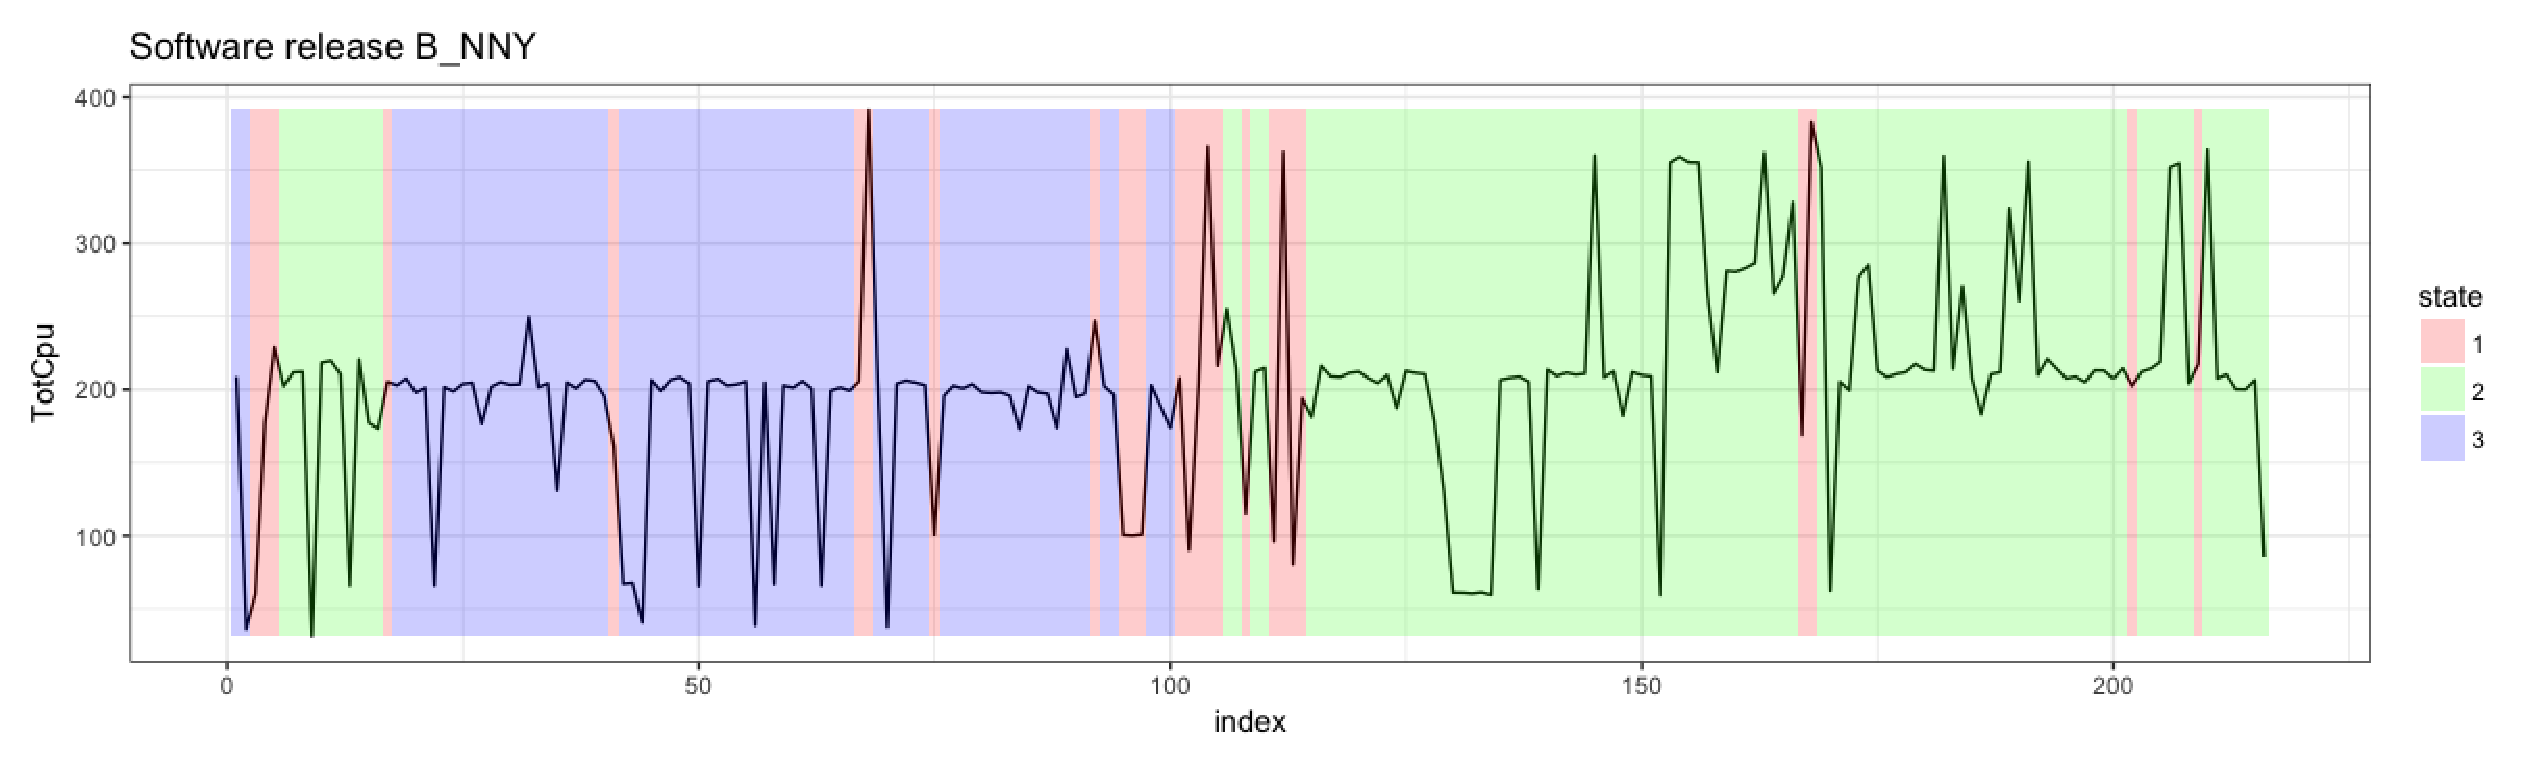
\includegraphics[scale=0.35]{picture/L16B_NNY1}
\par\end{centering}
\caption{The CPU utilization of the software release L16B showing the periods
where the observation is in the specific state. \protect \\
Model 2: DuProdName and Fdd/Tdd are non-switching coefficients.}
\label{L16B_NNY}
\end{figure}


